\section{Design}
\label{sec:design}

The data paths in our examples suggest a strategy to meet our design challenges.
There are recurring logical ``gateways'' that
connect the application and underlying components
(Figure~\ref{fig:deployment}).  Written data flows from the
application to the cloud storage provider through a storage-facing
gateway, external data flows from dataset providers to the application
through a dataset-facing gateway, and data flows between application
endpoints through cache-facing gateways.

Our strategy is to design these gateways as a wide-area storage service that address common 
storage concerns, while also allowing for application extensibility.
In doing so, we let the developer focus on implementing
domain-specific storage functionality, while internally handling
consistency, fault-tolerance, and security at scale.

%llp - a continuation of my comments at the end of the previous
%section... this focus on gateways as the key is fine, but seems
%to dimension some other aspects; e.g., how we "divert" data through
%caches, and how we maintain consistency in the face of caching.
% (This is at the big-picture/overview level... there are plenty of
%details that follow, but this gateway-heavy lead might cause readers
%to miss these other key ideas.

\subsection{Abstractions and Components}

\Syndicate\ must distinguish between the application's data records
in order to apply the domain-specific storage functionality to them.  At the same time, it must allow
the application to structure and search its records efficiently, in
a way that is not coupled to an underlying provider's semantics.

To do so, \Syndicate\ defines three data abstractions:
\textit{objects}, \textit{directories}, and \textit{Volumes}.  Objects
store record data and are similar to files, but contain extra metadata used to
programmatically control the storage functionality applied to them.
For example, developer-given code can extend \Syndicate\ to impose internal structure 
on object data.  Objects are organized hierarchically by directories, making them efficiently organizable
and searchable by applications.

A Volume binds a rooted tree of directories to a set of providers and a set of principals,
one of which is the Volume's owner.  Within a Volume, an object's data can be distributed 
across one or more providers, and accessed by one or more principals. 

To present these abstractions to applications, \Syndicate\ provides \textit{\Syndicate\ gateways}
(\SGs), peer processes which coordinate via a scalable cloud-hosted {\it Metadata Service} (\MS).
\SGs\ are the first-class analogues of the logical gateways discussed earlier.

The \SG\ comes in three variants, based on how it interfaces with external providers.
They all play the same role in the larger \Syndicate\ design, and so we do not
distinguish between them unless critical to understanding the system.

\begin{description}

\item[\bf User \SG:] Interfaces with edge caches for an application endpoint.
  Responds to application read/write requests, read requests from edge caches,
  and read/write requests from peer \SGs.  Our
  prototype offers four instances: a
  FUSE~\cite{fuse} filesystem, a Web
  object store, a Python library, and a Hadoop Filesystem~\cite{hdfs}.

\item[\bf Replica \SG:]  Interfaces with cloud storage providers.
  Responds to read/write requests from peer User \SGs, but does not generate
  any requests of its own.  Acts as an origin server for edge caches for cloud-hosted data.  Our prototype
  currently supports Amazon S3 and Glacier~\cite{aws-overview}, Dropbox~\cite{dropbox},
  Box.net~\cite{Box.net}, Google Drive~\cite{google-drive}, and local disk.

\item[\bf Acquisition \SG:]  Interfaces with dataset providers.  Maps an existing dataset
  into a Volume as a read-only directory hierarchy.  Acts as an origin server for edge caches
  on behalf of the dataset provider, and does not generate any local requests.  Our prototype currently supports
  local filesystems and SQL-speaking RDBMSs, and can generate data dynamically using 
  dataset-specific tools.

\end{description}

\begin{figure}[h!]
\centering
\includegraphics[width=0.45\textwidth]{figures/Syndicate-fig}
\caption{\it Logical positioning of \Syndicate\ Gateways (\SGs) between edge caches, cloud storage (DropBox, S3), datasets, and application logic.}
\label{fig:deployment}
\end{figure}

The \MS\ helps \SGs\ coordinate globally. It maintains the authoritative
state of each Volume's metadata, and helps the system scale, tolerate
faults, and keep data consistent.  The \MS\ binds each \SG\ to one
Volume, and helps \SGs\ discover their peer \SGs.

In a typical deployment, an application 
uses one \MS, and places data in objects distributed across one or more Volumes.
Application endpoints run User \SGs\ locally to access Volume data, and 
the developer provisions other \SGs\ to attach cloud storage and external datasets.
The developer also has options for attaching an existing set of principals to a Volume
(Section~\ref{sec:security}), facilitating integration with existing organizations.

\subsection{Object Data}

The \SGs\ execute an extensible read and write protocol to handle application reads 
and writes in a way that is not coupled to the underlying providers.  We present the
protocols here, and discuss their extensibility in Section~\ref{sec:composition}.

Each object is assigned an \SG\ that acts as its {\it coordinator}, which handles reads and writes
to it from other \SGs\ and edge caches.  \Syndicate\ lets application control this assignment,
and control post-read and pre-write processing (Section~\ref{sec:composition}).

\SGs\ read data from each other using their Volume's edge cache providers.
This allows the application to transparently benefit from the data locality they offer,
as well as scale up the number of reads it can handle.
However, reading fresh data from them is difficult because
each cache provider offers different functional semantics regarding 
cache control and consistency directives.  For example, a cache provider might
impose a minimum cached object lifetime to prevent clients from accidentally 
overwhelming an origin server.

\Syndicate\ obviates the need for these directives by ensuring each URI
uniquely identifies a snapshot of data.  The challenges in doing so
are to use cache capacity efficiently (to avoid thrashing),
and ensure \SGs\ discover the correct URIs before downloading.

To address the former, \SGs\ serve object data as blocks.
This lets edge caches evict data block by block, subject to their own eviction policies.
The block size is chosen by the developer based on the application's workloads; \Syndicate\
helps this choice by reporting internal fragmentation rates.

To address the latter challenge, an \SG\ stores a 
generation nonce and last-modified nonce for each
object it coordinates.  The generation nonce is assigned 
on creation, and the last-modified nonce is assigned when the last successful write 
is processed.  For each block in each object, the \SG\ additionally stores a block nonce 
that identifies its current contents, as well as the set of \SGs\ in the Volume that 
can serve a replica of it.  It keeps track of this information using an object
\textit{manifest} (Figure~\ref{fig:manifest}), and uses this information
to generate block URIs.  The \MS\ stores copies of each object's generation
and last-modified nonces.

\begin{figure}[h!]
\centering
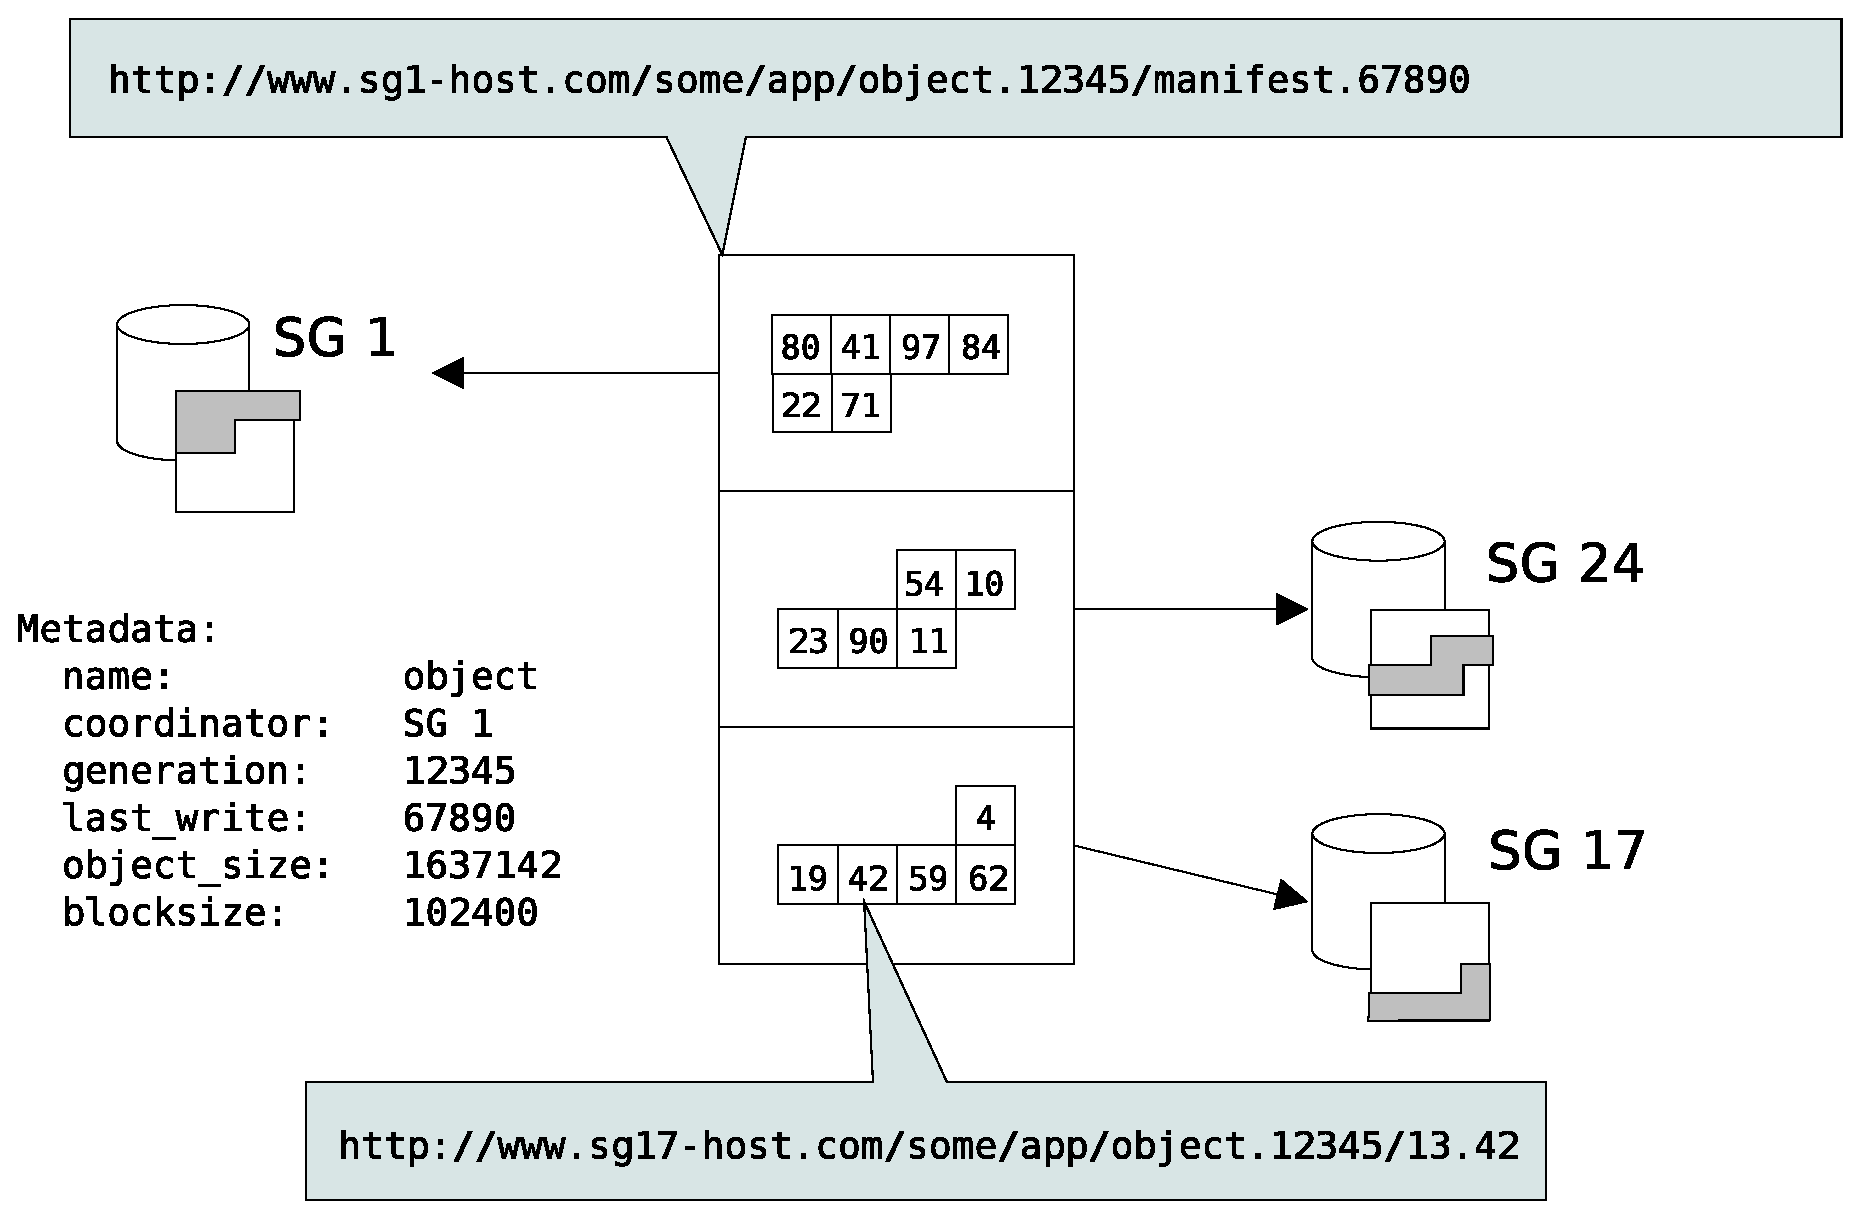
\includegraphics[width=0.47\textwidth]{figures/manifest}
\caption{\it Logical representation of a manifest for a 16-block object after 
three writes.  Each \SG\ (cylinders) hosts the latest 
copies of some of the object blocks (grey areas), which the manifest tracks.  (Generation nonces,
last-modified nonces, and block nonces are kept short in this figure for brevity.)}
\label{fig:manifest}
\end{figure}

The \SG\ reads an object's data by first obtaining a fresh object manifest, and then 
obtaining the desired blocks (Figure~\ref{fig:protocols}).
To get a fresh manifest, the \SG\ first obtains the
object's generation and last-modified 
nonces from the \MS.  It uses them, along with the object's path,
to generate an URI for the manifest.  By including them,
the URI identifies a manifest snapshot as fresh as the nonces,
allowing it to use edge caches to obtain fresh manifest data.

Once obtained, the \SG\ uses the manifest to build 
URIs for each block.  A block URI
includes the object's path, generation nonce,
the block offset, and the block nonce.  This allows 
it to download block data from edge caches that is guaranteed to be
as fresh as the manifest.

The write protocol (Figure~\ref{fig:protocols})
is designed to let \Syndicate\ scale write bandwidth and tolerate
\SG\ failures while allowing the
application to control data formatting and inter-object
write ordering.  When an \SG\ writes to an object, it first obtains
a fresh manifest, generates the new blocks
and block nonces, and sends them to a Replica \SG.  It includes the object ID,
generation nonce, and last-modified nonce, so the Replica \SG\ can uniquely
identify each block (so it can be garbage-collected when overwritten).

The writer sends the block nonces
to the coordinator.  Upon receipt, the coordinator generates a last-modified
nonce, adds the block nonces to its manifest, and uploads the manifest to 
a Replica \SG.  It then sends the object last-modified nonce
to the \MS, so subsequent readers can discover it.
It finally acknowledges the writer \SG, and
asynchronously garbage-collects overwritten blocks from the Replica \SGs.
Each User \SG\ logs each step of the write to local stable storage, so it can
roll back a write or garbage-collect data if it fails and restarts during the operation.

\begin{figure}[h!]
\centering
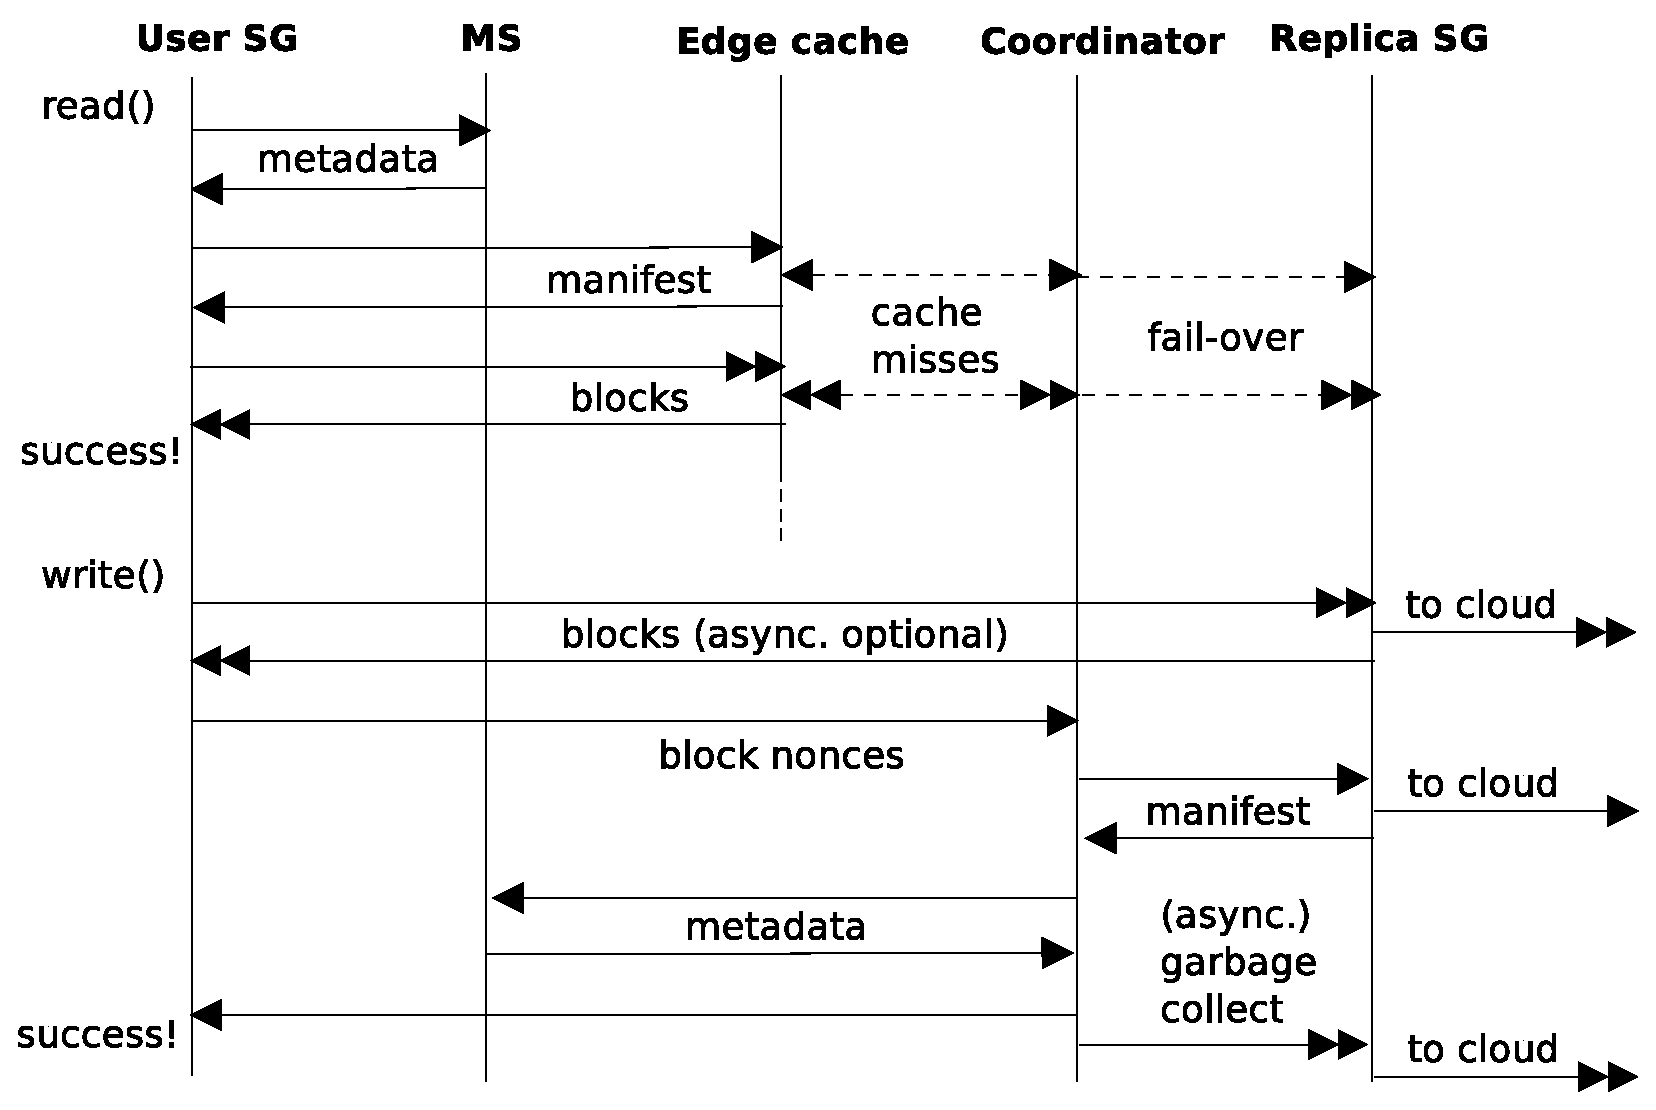
\includegraphics[width=0.47\textwidth]{figures/protocols}
\caption{\it Protocol overview for reads and writes.  Some steps are performed asynchronously, as marked.}
\label{fig:protocols}
\end{figure}

\subsection{Object Metadata}
\label{sec:metadata-consistency}

Where data plane operations are 
concerned, the \SGs\ rely on the \MS\ to
announce their presence and the objects they coordinate,
to discover other \SGs\ and objects, and to help them download fresh
object data from one another.

The \MS\ maintains a metadata record for every object/directory in 
each Volume, as well as records for each \SG.
A metadata record is functionally similar to an i-node;
a listing of relevant fields the 
\MS\ tracks can be found in Table~\ref{tab:metadata}.
\SGs\ download and cache these records whenever they 
access an object for an application.

\begin{table}[ht!]
\begin{tabular}{ | l | l |}
\hline
\textbf{Name} & \textbf{Description} \\
\hline
\texttt{type} & Object or Directory record.\\
\texttt{name} & Object name. \\
\texttt{object\_id} & Volume-wide unique object ID. \\
\texttt{principal\_id}  & ID of the app principal that owns this object. \\
\texttt{coord\_id} & ID of the coordinator \SG. \\
\texttt{volume\_id} & Which Volume contains this object.\\
\texttt{generation} & Object generation nonce. \\
\texttt{last\_mod} & Object last-modified nonce. \\
\texttt{perms} & Permissions for this object. \\
\texttt{read\_ttl} & Cached metadata lifetime. \\
\texttt{write\_ttl} & Metadata write-back delay. \\
\hline
\end{tabular}
\caption{\it Partial list of record fields in the Metadata Service.}
\label{tab:metadata}
\end{table}

The \MS\ serves as coordinator 
for all directories, in order to serialize object/directory creation
and deletion in a single 
directory.  This ensures each path refers to one object,
so a read does not combine blocks from different objects.

\subsection{Programming Model}
\label{sec:composition}

The goal of our protocol designs is to isolate provider-specific logic from 
provider-agnostic logic, while letting the developer control 
how \Syndicate\ processes application data.
To achieve this, each \SG\ provides an event-driven programming model, where the developer implements 
a set of callbacks that operate on an application request (Table~\ref{tab:api}).
The developer writes code and configuration for the application's
 \SGs, and uses the \MS\ to automatically distribute it to them.

\begin{table*}[ht!]
\begin{tabular}{ | p{2in} | p{3in} | p{1.5in} |}
\hline
\textbf{User \SG} & \textbf{Replica \SG} & \textbf{Acquisition \SG} \\
\hline
\texttt{connect\_cache(): socket} & \texttt{read(request), get(key): bytes} & \texttt{manifest(m,obj): int} \\
\texttt{write\_preup(data): int} & \texttt{write(request,data), put(key,data): bool} & \texttt{read(block): int} \\
\texttt{read\_postdown(data): int} & \texttt{erase(request), del(key): bool} & \texttt{publish(spec): int} \\
\texttt{chcoord\_begin(obj): int} & & \\
\texttt{chcoord\_end(obj,status): int} & & \\
\hline
\end{tabular}
\caption{\it Programmatic interface overview for each Syndicate Gateway.  The Replica \SG's interface has a
provider-agnostic half (read(), write(), erase()) and a provider-specific half (get(), put(), del()).  }
\label{tab:api}
\end{table*}

An \SG's configuration is split into built-in state,
application-supplied state, secret state, and object attributes.  Built-in state 
includes ``inventory'' information, such as its public key, its application-chosen name,
its host and port, and its owner's ID.

Application-supplied state includes key/value pairs defined by the 
developer, which have extension-specific interpretations.  Secret state includes 
key/value pairs that are sealed with the \SG's public 
key before being pushed out, thereby ensuring that only the target \SG\ can read them.
For example, the developer's credentials to a 
cloud storage provider would be distributed as secret state to the appropriate Replica \SG.

Object attributes are key/value pairs 
that are defined per-object.  They are readable and writable only
to authorized User \SGs\ and the \MS\ (discussed in Section~\ref{sec:consistency}).

When a method is called on an object, it has access to all of the above configuration,
as well as internal methods within the \SG\ (not described here). 
It also has access to local code libraries, local storage, and its own 
private RAM for storing soft state across calls.

{\bf User \SG\ API}.  User \SG\ code opens connections to edge cache
providers (\texttt{connect\_cache()}), and applies application storage logic
to data before uploading it (\texttt{write\_preup()}) and after downloading
it (\texttt{read\_postdown()}).  This gives the application a 
chance to apply end-to-end storage logic (such as encryption and formatting) on the data without 
having to deal with scalability and fault tolerance.  These methods are called for 
both manifest and block data.

The User \SG\ calls \texttt{chcoord\_begin()} and \texttt{chcoord\_end()} before 
and after becoming an object's coordinator.
This lets application control initial object distribution, and how and when to change it (for example,
an application may require popular objects to be pinned to highly-available \SGs).
The application can explicitly set an object's coordinator,
and \Syndicate\ can try to change it (subject to these methods) to tolerate faults and distribute load.

{\bf Replica \SG\ API}.  The Replica \SG\ serves manifest and block data to edge caches,
and uses its storage logic to access blocks and 
manifests in storage providers. It divides its functionality into both
provider-agnostic (\texttt{read(),write(),erase()}) and provider-specific (\texttt{get(),put(),del()})
logic, in order to make the former reusable while allowing the latter 
to be designed just once.  Unlike the others, Replica \SG\ methods must be
idempotent, so \Syndicate\ can automatically retry failed writes and deletes.

{\bf Acquisition \SG\ API}.  The Acquisition \SG\ serves blocks 
and manifests to edge caches automatically, but imposes no constraints on
how to acquire data from the dataset provider.  Its
logic translates arbitrary datasets into a directory hierarchy according to
a given specification, and uploads the directory 
tree to the \MS\ (via \texttt{publish()}) when it initializes.
The specification is provided by the data curators,
so they can white-list the ways in which the data can be
accessed by external parties (necessary when data is subject to
external usage policies, such as privacy laws).

Once it has published the data, the Acquisition \SG\ translates
manifest and block requests into the appropriate calls to the dataset provider
(\texttt{manifest()} and \texttt{block()}).
Because data may be dynamically generated, it does not 
report object sizes immediately, nor does it reply immediately with data.
Instead, it may send the User \SG\
an EOF message for block offsets that are logically beyond the end of the object,
and a ``try again later'' message for requests that will take a long time.
The User \SG\ handles both messages transparently to the application.

\subsubsection{Point-Solutions, Revisited}

To demonstrate the power of this programming model, we briefly sketch
solutions to the three application domains we described earlier.  A
scientific data-processing application can implement the Replica \SG's
provider-agnostic interface to snapshot and stage gene sequences for a
particular organism, such that continuous updates from grid computers
and collaborators do not corrupt cloud-hosted data being accessed by
compute nodes.  It can implement the Acquisition \SG's interface to
export data in legacy on-site storage as a Volume for collaborators to
access.

A collaborative document-sharing application can store documents as objects, and
store a document schema as an object attribute. It can implement the User \SG\ interface
to impose the schema's structure and content requirements for the associated document objects.
At the same time, it can implement end-to-end document
encryption to keep fields private from providers and users, using an object attribute 
to hold the shared secret (which is protected by \Syndicate's built-in access controls,
as described in the next section).  To efficiently ensure durability in the face of 
changing sets of providers, the Replica \SG's provider-agnostic interface can 
be implemented to store erasure codes to multiple providers instead of full replicas.

A VDI application can implement the User \SG\
interface to prompt for additional credentials, in order to authenticate to an 
in-house identity service prior to downloading the VM image.
It can distinguish between system and user partitions in the disk image, so it  
can request the former from shared caching infrastructure (since many users 
share it) and cache data from the latter to local disk.

\subsection{Default Consistency and Access Control}
\label{sec:consistency}

Unless explicitly overwritten by the developer in an \SG's extension,
\Syndicate\ offers built-in default consistency and access controls.
This lets developers rapidly deploy new storage functionality 
without repeatedly addressing common cases of these concerns.

Similar to edge cache control directives, the application controls both
how long (in wall-clock time) cached object metadata
is considered fresh in the User \SG\ (via \texttt{read\_ttl}), and how long to wait before uploading 
new object metadata on write (\texttt{write\_ttl}).  Values of zero make 
metadata access synchronous, and larger values reduce amortized access latency at the 
expense of data consistency.  In addition, \Syndicate\ offers last-write-wins
semantics by default for both data and metadata, and the application
controls whether or not data is ``flushed''
on write or via an explicit \texttt{fsync()} request.

In doing so, \Syndicate\ offers four built-in consistency models.
When both metadata access and writes are synchronous,
objects have sequential consistency.  But if writes are asynchronous, 
objects have close-to-open consistency.  If metadata access is asynchronous and
writes are synchronous, the object has delta consistency.
If both metadata access and writes are asynchronous, 
the object's consistency is determined
by the order in which the application flushes writes.

By default, \Syndicate\ ensures that a User \SG\ cannot 
discover objects that it cannot access.  The \MS\ uses the
\texttt{perms} field to determine whether or not a User \SG\ can read, write, or search
an object or directory.  Similar to POSIX permissions, these permissions apply based on whether or not 
the User \SG\ is running on behalf of the principal that created the object (akin to ``owner'' permissions),
whether or not it is the coordinator for the object (akin to ``group'' permissions), and
whether or on it is in the same Volume as the coordinator (akin to ``world'' permission).  The Volume owner also sets
Volume-wide capabilities for User \SGs---namely, to write data, to
read or write metadata, and to coordinate writes.  These preempt object permission bits,
and apply to object attributes as well.

At a higher level, Volumes can be marked as ``private,'' meaning that a User \SG\ must prove that
it is acting on behalf of an authorized principal (as opposed to ``public,'' which 
allows anonymous read-only access).  They may also be marked as serving as an 
``archive,'' meaning that they are read-only to every \SG, except for
Acquisition \SGs\ owned by the Volume's owner.  This lets
external dataset providers export data for \Syndicate's consumption, without 
clobbering objects.

These access controls determine how \SGs\ can alter the state of the Volume,
and are enforced on top of of application-supplied logic by default.
However, they do not prevent direct access to object data via providers;
the application should implement end-to-end encryption in the User \SG\ if this 
is a concern.

\subsection{Scalability and Fault Tolerance}
\label{sec:controlplane}

Regardless of application-supplied storage functionality, \Syndicate\ must
transparently scale in the number of \SGs\ and number of writes while tolerating
failures in both.  To manage \SGs\ at scale,
\Syndicate\ treats code and configuration like objects,
allowing \SGs\ to use edge caches for scalable distribution.  \SGs\ exchange
last-modified nonces for the set of code and configuration
via an asynchronous gossip protocol, so new versions pushed to the \MS\ are quickly 
discovered and pulled.  They are signed with the Volume's private key to prove authenticity and integrity.

A logically-single Replica \SG\ can be instantiated multiple times to scale write bandwidth,
either alongside each User \SG, or in a cluster behind a load-balancer.
Because its storage methods are idempotent,
User \SGs\ can retry or roll back failed writes regardless of instantiation.

\Syndicate\ scales aggregate write load by dynamically distributing objects across
User \SGs.  At first, an object's coordinator is the \SG\ that created it.
If it becomes unavailable, or the application changes it, a candidate \SG\
(i.e. a subsequent writer User \SG\ or the application's new choice)
will ask the \MS\ to become the new coordinator.  To do so, it
submits the current object generation nonce with the request, and the \MS\
atomically regenerates it on success.  This forces
other candidates to refresh the object metadata,
causing them to learn the new coordinator before they try again.
This also causes writer \SGs\ that cannot contact each other to ``take turns'' coordinating,
keeping objects available for writes in the face of such partitions (albeit 
with degraded performance).

Without being given extra functionality for doing so, an \SG\ cannot make progress if the \MS\ is inaccessible.
This is equivalent to a non-\Syndicate\ application losing access to its providers.
However, the \MS\ implementation is portable across multiple cloud platforms,
so the application developer can choose the platform that offers the best availability/cost
trade-off.

\subsection{Security}
\label{sec:security}

At all times, \Syndicate\ must provide a storage layer which the application 
can trust to enforce access control, authenticate principals, and distribute its extensions.
Our threat model assumes that eavesdroppers (Eve) read data on the network and within providers, but not 
within \Syndicate\ components, TLS CAs, or the \MS's underlying storage.  We also assume that malicious 
agents (Mal) try to spoof the \MS\ and \SGs, and try to compromise running \SGs.
\Syndicate\ thwarts Eve with end-to-end encryption, and limits the damage 
Mal can do by enforcing built-in access controls and detecting attempted spoofs.

A Volume acts as a virtual certificate authority and key repository for
its \SGs.  It maintains a signed certificate for each authorized, non-anonymous \SG, 
each of which cryptographically binds the \SG\ to its Volume and configuration (including
its public key, capabilities, host, and port).  If desired by the developer, it also 
hosts a copy of the encrypted private key
for each \SG\ (accessible only after the \SG\ authenticates), which is automatically
generated, sealed, and uploaded when the \SG\ is provisioned.

Each \SG\ maintains a certificate bundle for all other \SGs\ in the same Volume.
To distribute it at scale, \Syndicate\ represents it as an object,
where each certificate is a ``block.''
The \MS\ and \SGs\ gossip its cryptographic hash and last-modified nonce,
and automatically re-synchronize the bundle if it changes.  Unlike a typical 
``object'', the last-modified nonce of the certificate bundle increases monotonically,
so \SGs\ can detect stale bundles submitted by Mal.

To ensure the application can trust the storage layer created by the running \SGs,
\Syndicate\ puts it in charge of bootstrapping the trust on a per-session basis.
When the developer starts an \SG, she gives it login
credentials to use to register itself with the \MS, as well 
as its private key decryption password.  The \SG\ 
submits the login credentials (via TLS) to a developer-chosen OpenID~\cite{openid} provider,
which the \MS\ is configured to trust
(i.e. either a 3rd party one, or one built into the application logic).
Once the OpenID provider vouches for the authenticity of both components,
the \SG\ obtains its encrypted private key and decrypts it locally.

While running, \Syndicate\ uses TLS to keep control-plane messages
confidential and to prevent replay attacks from Mal.  Each message is
signed by the sender, allowing it to ignore Mal's unverifiable
messages.  To keep Mal from silently altering data in a provider, a coordinator
signs each manifest; since the manifest contains the block's cryptographic hashes,
a reader \SG\ can detect tampering.

A compromised User or Acquisition \SG\ is limited to damaging only its
Volume, and only as far as \Syndicate's built-in access controls allow
(provided that an application-supplied extension does not weaken them).  The
\MS\ always forbids a Replica \SGs\ from altering Volume metadata, but
a compromised Replica \SG\ can destroy data.  Application developers
hedge against data loss by using multiple Replica \SGs\ linked to
different storage accounts in different providers.

